% !TEX root = ../Ausarbeitung.tex
\section{Funktionalität von Containern}
\label{sec:Funktionalität von Container}

Container setzen direkt auf dem Kernel eines Linux-Betriebssystems auf. Um auf den Kernel durchgreifen zu können, verwenden Container standard-Linux-Techniken wie Cgroups und Namespaces oder selbst entwickelte Schnittstellen. Dadurch wird das Betriebssystem innerhalb des Containers, ohne vollständige Virtualisierung emuliert. Die folgende Grafik verdeutlicht den Kernelzugriff:
\begin{figure}[H]
	\begin{center}
		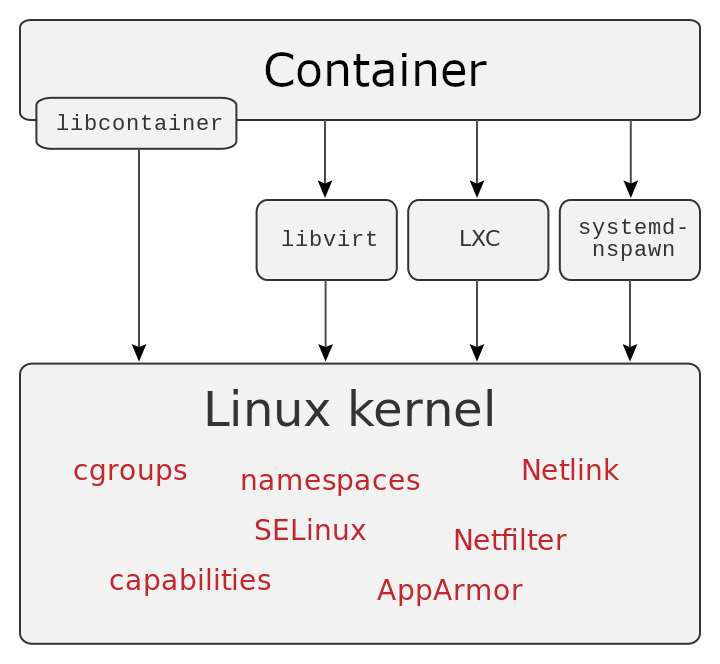
\includegraphics[width=0.7\textwidth]{LinuxKernelContainer.png}
	\end{center}
	\caption[Schnittstelle vom Container zum Kernel]{Schnittstelle vom Container zum Kernel \footnotemark}
	\label{fig:HW1}
\end{figure}
\quellefoot{4}{https://www.datacenter-insider.de/container-technik-docker-co-a-480855/index2.html}
Somit können CPU-Zyklen, Arbeitsspeicher, Blockspeicher und sonstige Schnittstellen über den Kernel angefordert und isoliert in dem jeweiligen Container zur Verfügung gestellt werden.\cite{DataCenter}

Da sie nur als einzelnes Image abgelegt sind, und kein Betriebssystem beinhalten, welches aktualisiert und gewartet werden müsste, beschränken sich die Installation und Deinstallation auf ein einfaches kopieren oder löschen des Containers. 
Aus einem Image können beliebig viele Container-Instanzen aufgerufen werden, da Schreibzugriffe nicht auf das Image auf das Image zugreifen sondern auf ein eigenes Dateisystem des Containers. Dieses Verhalten sorgt für eine sehr hohe Skalierbarkeit, da bei Bedarf einfach neue Instanzen der Anwendung gestartet werden können.\cite{DevInsider}
